\chapter{KIỂM THỬ VÀ KẾT QUẢ}

\section{Chiến lược kiểm thử}
\TODO{TV2/TV4. Unit $\rightarrow$ co-sim ISS $\rightarrow$ bộ test hazard $\rightarrow$ \texttt{system\_tb} (G1 và G2, có/không ngắt) $\rightarrow$ màn hình ảo; kiểm thử đột biến. Số kiểm lấy từ hồi quy mới nhất trong \texttt{evidence/}. Nháp màn ảo: \texttt{report/3.1-man-ao.md}.}

\section{Trace và dạng sóng}
\hinhtrong{Dạng sóng: load-use bubble, flush nhánh, \texttt{busy} freeze, vào/ra ngắt (H8)}{TV3}{4 ảnh, chú thích chu kỳ khớp \texttt{pipeline-policy.md} §7}

\section{Hiệu năng G1 và G2: CPI tách theo nguyên nhân}
\TODO{TV2/TV3. Số đếm bằng \texttt{tools/cpi.py}, không ``$\approx$''. Nháp: \texttt{report/3.3-cpi.md}.}

\section{Khảo sát thiết kế (DSE) và tài nguyên}
\TODO{TV1. Nháp: \texttt{report/3.4-dse.md}; còn thiếu phần tài nguyên (plan §8.2).}
\begin{figure}[htbp]\centering
  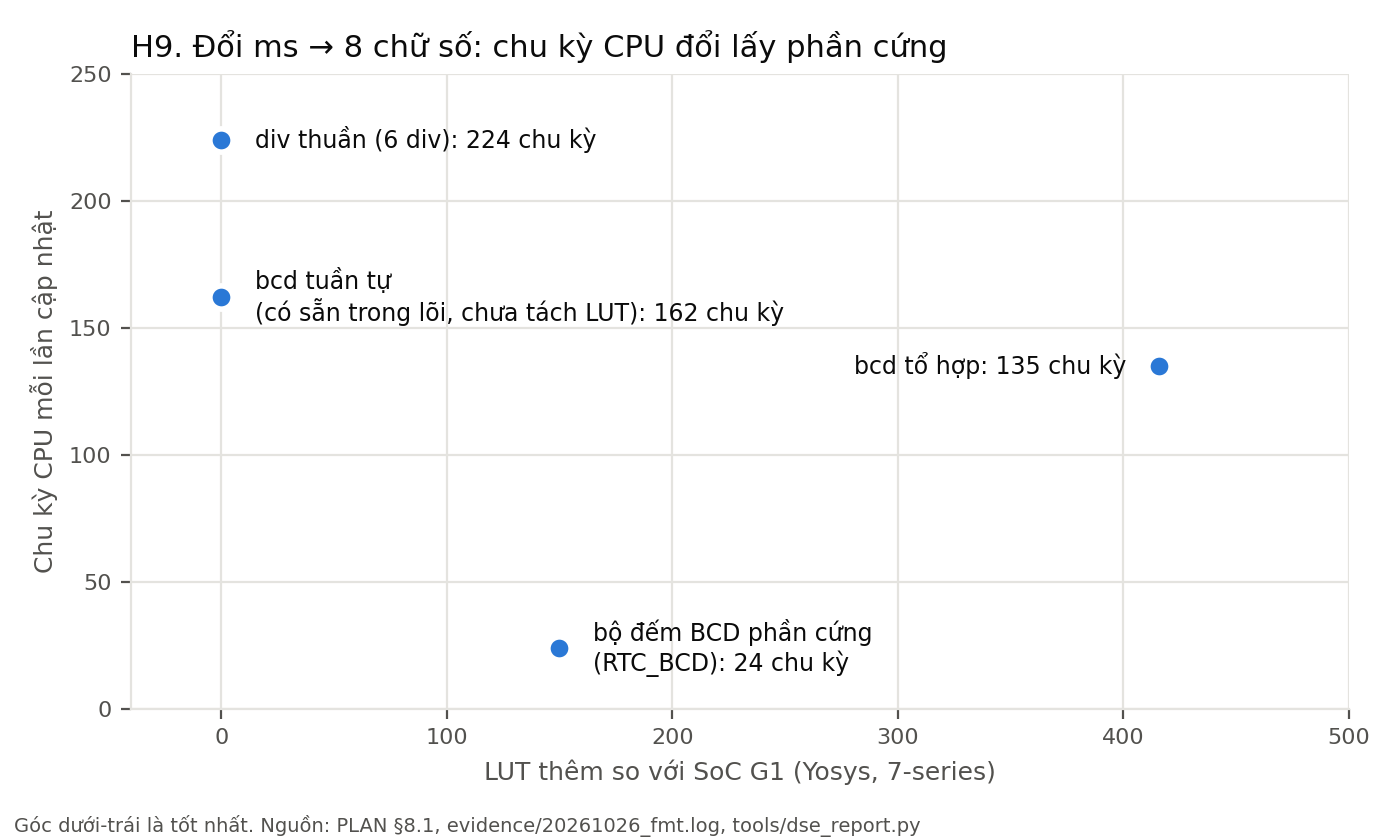
\includegraphics[width=0.85\linewidth]{h9_dse}
  \caption{Chi phí đổi ms sang chữ số (H9)}
\end{figure}

\section{Thí nghiệm E1$'$--E4$'$}\label{sec:thi-nghiem}
\TODO{Mỗi thí nghiệm: câu hỏi $\rightarrow$ cách đo $\rightarrow$ bảng/hình $\rightarrow$ kết luận + phạm vi đúng. Trả lời câu hỏi ``chuẩn ms'' của chương 1.}
\subsection{E1$'$, E2$'$: hiệu chỉnh CAL}
\TODO{TV5. Nháp: \texttt{report/2.4-cal-thi-nghiem.md}.}
\subsection{E3: polling, ngắt và capture}
\TODO{TV3 + TV2. Nháp: \texttt{report/2.5-e3-thi-nghiem.md}.}
\subsection{E4$'$: bóng ma khi quét 7 đoạn}
\TODO{TV4. Nháp: \texttt{report/2.3-bongma-e4.md}. Kèm H10 (màn hình ảo).}
\begin{figure}[htbp]\centering
  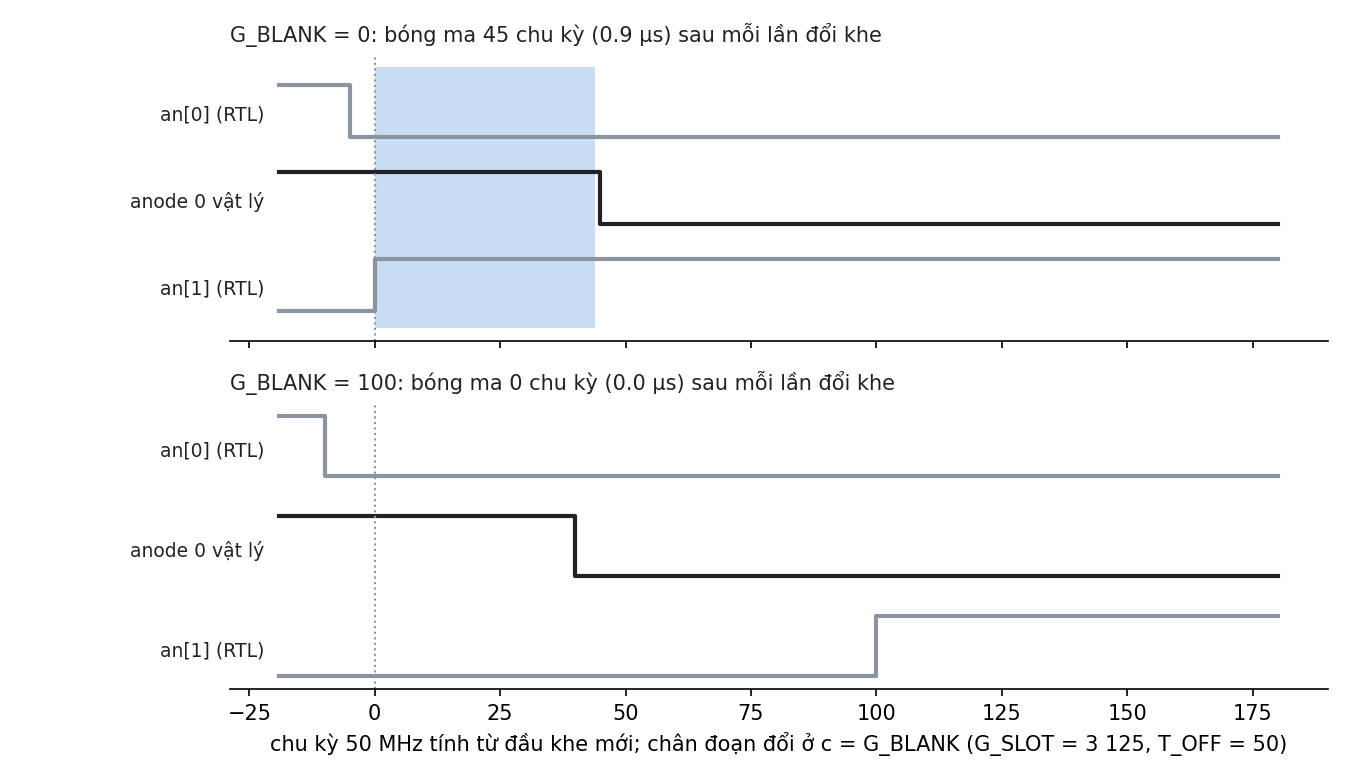
\includegraphics[width=0.85\linewidth]{h_e4_bongma}
  \caption{Bóng ma theo thời gian tắt của chân đoạn, ở 3 giá trị \texttt{G\_SLOT}}
\end{figure}

\section{Tổng kết: đạt và chưa đạt}
\TODO{TV2. Nháp: \texttt{report/3.6-bang-dat.md}. Mỗi dòng trỏ về 1 file \texttt{evidence/}; người viết tự chạy lại rồi mới tick.}
